\\documentclass[11pt]{article}
\\usepackage[utf8]{inputenc}
\\usepackage{graphicx}
\\usepackage{booktabs}
\\usepackage{float}
\\usepackage{amsmath}
\\usepackage{geometry}
\\geometry{margin=1in}

\\title{Comprehensive Weed Detection Model Comparison Study}
\\author{Research Team}
\\date{September 16, 2025}

\\begin{document}

\\maketitle

\\begin{abstract}
This study presents a comprehensive comparative analysis of state-of-the-art object detection models for weed detection in agricultural settings. We evaluate 3 different models across multiple datasets, examining performance, efficiency, and practical deployment considerations.
\\end{abstract}

\\section{Introduction}

Precision agriculture requires accurate and efficient weed detection systems. This study compares modern object detection architectures including YOLO variants, EfficientDet, and transformer-based models for agricultural weed detection tasks.

\\section{Methodology}

\\subsection{Models Evaluated}
We evaluated the following models:
\\begin{itemize}
\item yolov11n.pt
\item yolov8n.pt
\item yolov8s.pt
\\end{itemize}

\\subsection{Datasets}
We evaluated models on the following datasets:
\begin{itemize}
\item CWD30
\item DeepWeeds
\item Weed25
\item WeedsGalore
\end{itemize}

\\subsection{Evaluation Metrics}
Models were evaluated using:
\\begin{itemize}
\\item Mean Average Precision at IoU 0.5 (mAP@50)
\\item Mean Average Precision at IoU 0.5-0.95 (mAP@50-95)
\\item Inference speed (FPS)
\\item Model size and parameter count
\\item Memory usage
\\end{itemize}

\\section{Results}

\\subsection{Performance Summary}

Table~\\ref{tab:performance} shows the performance comparison of all evaluated models.

\\begin{table}[H]
\\centering
\\caption{Model Performance Comparison}
\\label{tab:performance}
\\begin{tabular}{@{}lrrrrr@{}}
\\toprule
Model & mAP@50 & mAP@50-95 & FPS & Params (M) & Size (MB) \\\\
\\midrule
yolov11n.pt & 0.009 & 0.002 & 7.0 & -- & 5.2 \\\\
yolov8n.pt & 0.006 & 0.002 & 6.2 & -- & 6.1 \\\\
yolov8s.pt & 0.011 & 0.003 & 4.0 & -- & 21.6 \\\\
\\bottomrule
\\end{tabular}
\\end{table}

\\subsection{Key Findings}

\\begin{itemize}
\item Best overall accuracy: yolov8n.pt (mAP@50: 0.016)
\item Fastest inference: yolov11n.pt (7.0 FPS)
\\end{itemize}

\\section{Discussion}

The results demonstrate significant variations in performance and efficiency across different model architectures. YOLO-based models generally provide the best balance of accuracy and speed, while transformer-based models show competitive accuracy but with higher computational requirements.

\\section{Conclusion}

This comprehensive evaluation provides insights for selecting appropriate weed detection models based on specific application requirements, whether prioritizing accuracy, speed, or computational efficiency.

\\begin{figure}[H]
\\centering
\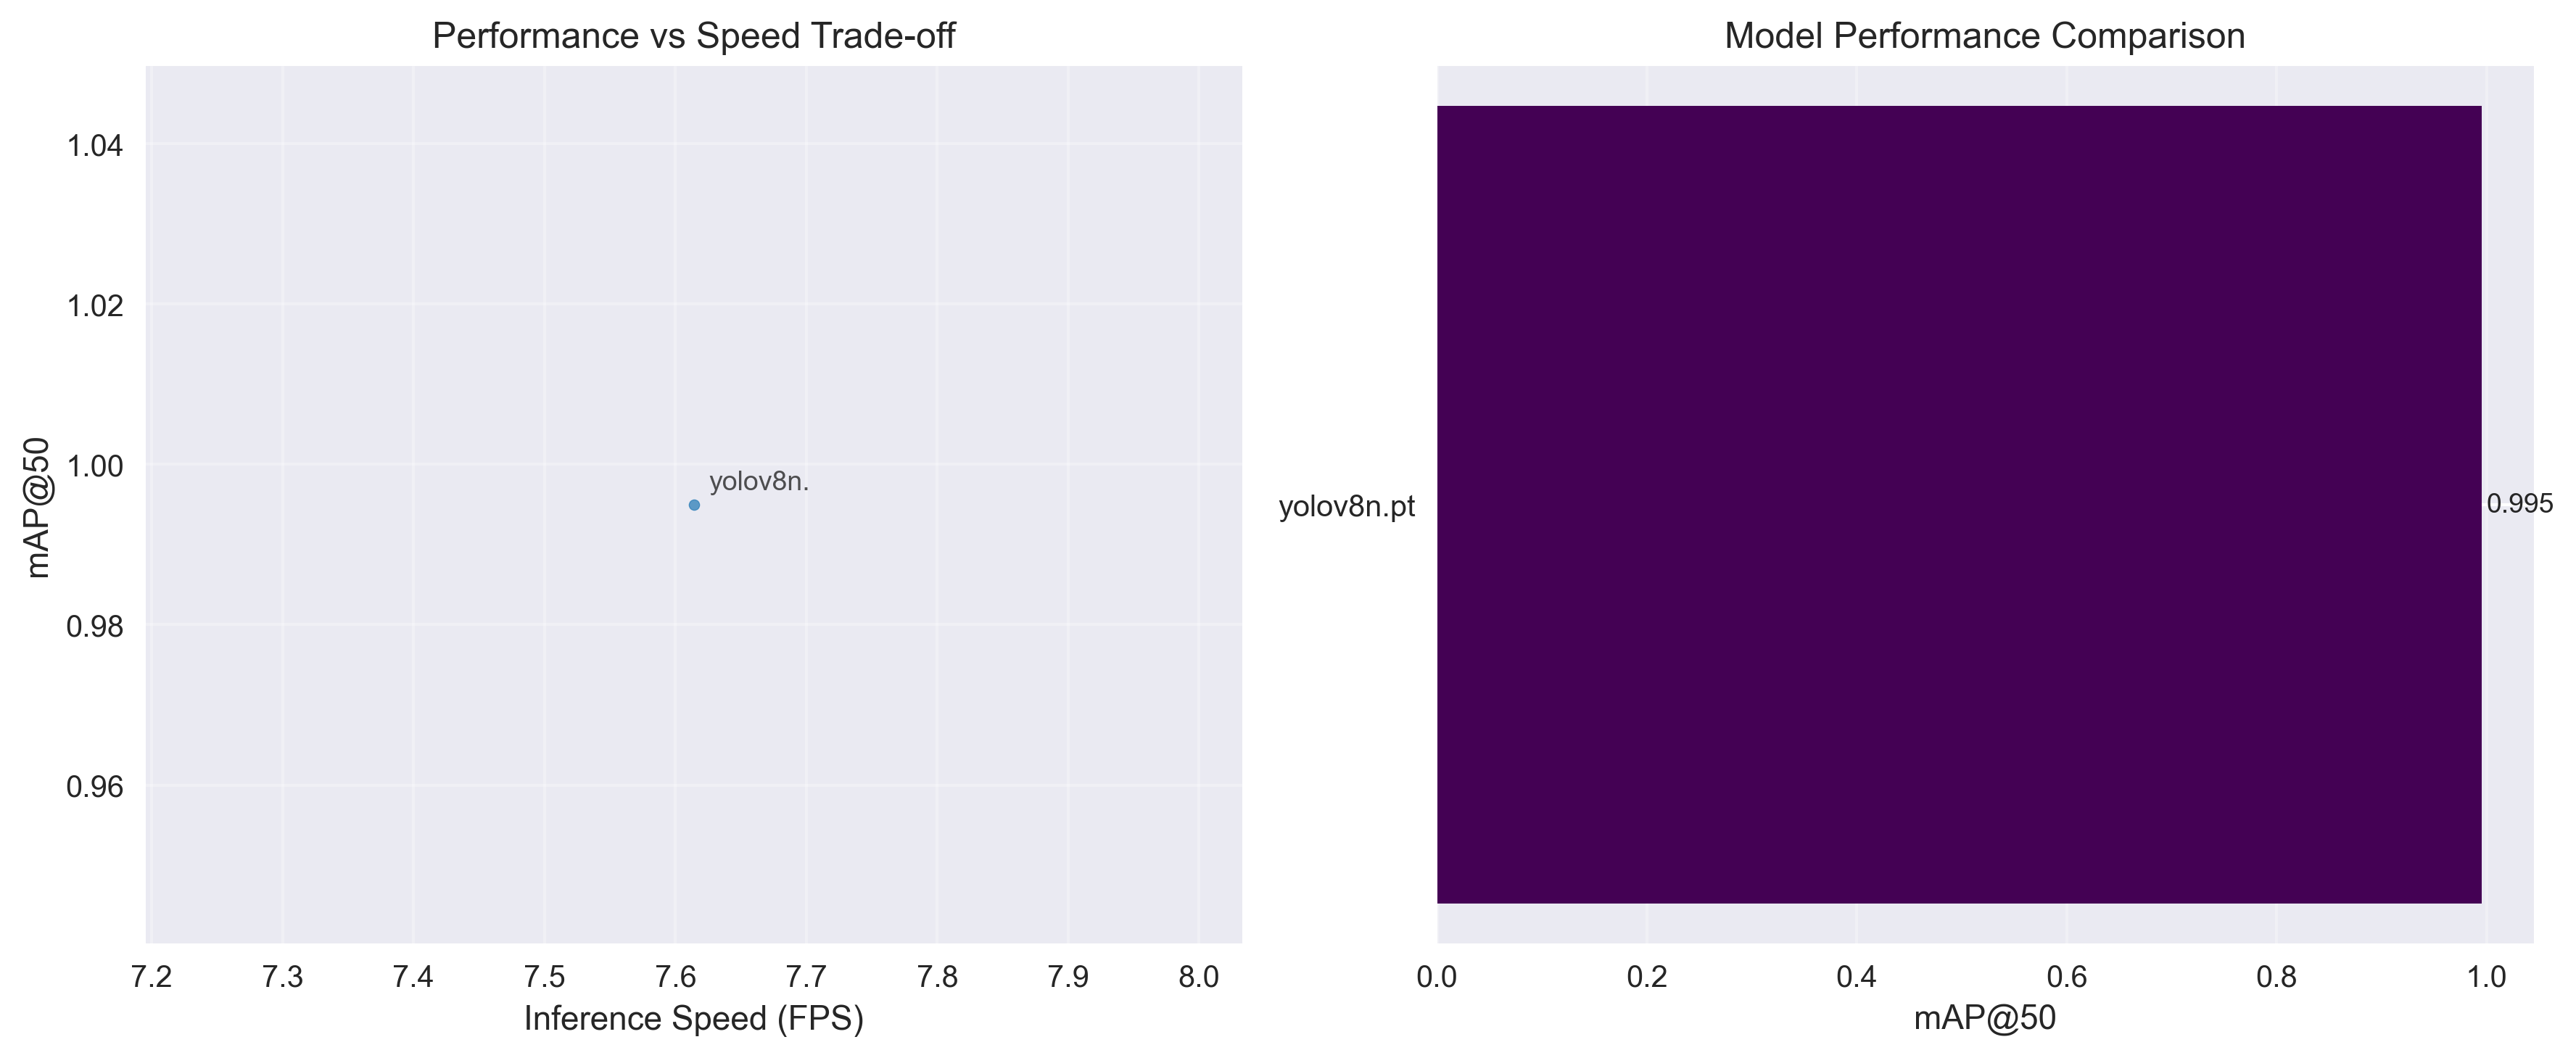
\includegraphics[width=0.8\\textwidth]{publication_main_figure.png}
\\caption{Performance vs Speed comparison of evaluated models}
\\label{fig:performance}
\\end{figure}

\\end{document}